\section{Multiphase Flow, eine Dimension mit 3 PDFs - untersucht von Dia} \label{sec:1d_simple}

Dia hat verschiedene Artikel in den letzten Jahren veröffentlicht, in
denen er analytische und numerische Berechnungen von Multiphase Flow
mit Riemann Randbedingungen durchführt. In diesem Kapitel soll das
einfachste System, 3 hyperbolische konservative partielle
Differentialgleichugen vorgestellt werden, wie sie in \cite{dia_2009}
und in seiner \cite{dia_diss} untersucht werden.
  
\subsection{Das Modell} \label{sec:3pdfs_1d}

In \cite{dia_2009} wird folgendes ein-dimensionales Modell zur Beschreibung
eines Gas-Flüssigkeit Systems vorgestellt
\begin{eqnarray}
\frac{\partial}{\partial t}\rho + \frac{\partial}{\partial x} \rho u
&=&  0\label{eq:dia_2009_k}\\
\frac{\partial}{\partial t} \rho u + \frac{\partial}{\partial x} (
\rho u^2 + \rho c (1-c) u_r^2 + P)&=& \rho g \label{eq:dia_2009_i}\\
\frac{\partial}{\partial t} u_r + \frac{\partial}{\partial x} (
uu_r + \frac{1-2c}{2} u_r^2 + \Psi(P)) &=& \frac{S^I}{\rho c
  (c-1)}. \label{eq:dia_2009_r}
\end{eqnarray}


Die Volumenanteile werden wieder mit $ \alpha_1$ und $\alpha_2,
\alpha_1+\alpha_2=1$ bezeichnet. Der Index 1 beschreibt die
Flüssigkeit, der Index 2 das Gas. Zur Reduktion der Indices wird
$\alpha_2=\alpha$ und $\alpha_1=(1-\alpha)$ gesetzt. Die Symbole
bedeuten

\begin{tabular}{rl}
$\rho = \alpha_1\rho_1 + \alpha_2\rho_ 2 = \alpha \rho_2 + (1-\alpha)
  \rho_1$ & gemittelte Dichte\\[3mm]
$c = c_2 = \frac{\alpha_2\rho_2}{\rho}, c_1 =
  \frac{\alpha_1\rho_1}{\rho} = 1-c$ & Gas-Massenanteil\\[3mm]
$u = \frac{\alpha_1\rho_1}{\rho} v_1 + \frac{\alpha_2\rho_2}{\rho} v_2  
   = c_1 v_1 + c_2 v_2$  & gemittelte Geschwindigkeit\\[3mm]
$u_r = v_2 - v_1$ & relative Geschwindigkeit\\[3mm]
$P$ & Druck für beide Phasen zusammen\\[3mm]
$\Psi(P)$ & verbindet die Phasen in der Impulsgleichung\\[3mm]
$g$ & Graviationskonstante\\[3mm]
$S^I$& Wechselwirkung zwischen den Phasen\\[3mm]
\end{tabular}

Die Geschwindigkeiten der einzelnen Phasen werden mit $v_1$ und $v_2$
bezeichnet und die Dichten mit $\rho_1$ und $\rho_2$.

{\bf 1. Kontinuitätsgleichung \ref{eq:dia_2009_k}}


Die Gleichungen lassen sich über die Eulergleichungen aus Kapitel \ref{subsec:Euler}
herleiten.  Die Kontinuitätsgleichung \ref{eq:dia_2009_k} stimmt mit
der Gleichung \ref{eq:fluent-mixed-konti} überein bzw. ist die Summe
der Gleichungen \ref{eq:eulerKonti} 
\[
\frac{\partial}{\partial t} (\alpha_i \rho_i)  + 
\frac{\partial}{\partial x} (\alpha_i\rho_i v_i) = 0 \quad i=1,2
\]
ohne Quelle und ohne Massenübergang von einer Phase in die andere,
also $\dot{m}_{12}=0$.
\begin{eqnarray*}
\frac{\partial}{\partial t} (\alpha_1 \rho_1)  + 
\frac{\partial}{\partial x} (\alpha_1\rho_1 v_1) 
+
\frac{\partial}{\partial t} (\alpha_2 \rho_2) + 
\frac{\partial}{\partial x} (\alpha_2\rho_2 v_2)  &=& 0\\
\frac{\partial}{\partial t} \rho + \frac{\partial}{\partial x} (\rho u) &=& 0
\end{eqnarray*}

{\bf 2. Impulsgleichung \ref{eq:dia_2009_i}}

Vergleicht man die Impulsgleichungen \ref{eq:fluent-mixed-impuls} mit
\ref{eq:dia_2009_i} bzw. \ref{eq:eulerImp}, so findet man auch
Übereinstimmung mit den addierten Euler-Gleichungen 
\[
\frac{\partial}{\partial t} (\alpha_i \rho_i v_i) + \frac{\partial}{\partial x} 
(\alpha_i\rho_i v_i v_i) = - \frac{\partial}{\partial x} \alpha_i P_i +
\alpha_i\rho_i g \quad i=1,2
\]
ohne Spannungstensor und ohne weitere Kräfte:
\begin{eqnarray*}
\frac{\partial}{\partial t} (\alpha_1 \rho_1 v_1 + \alpha_2 \rho_2 v_2) +
\frac{\partial}{\partial x} (\alpha_1 \rho_1 v_1 v_1 + \alpha_2 \rho_2 v_2 v_2) 
&=& 
- \frac{\partial}{\partial x} (\alpha_1 P_1 + \alpha_2 P_1)
+ g (\alpha_1\rho_1 + \alpha_2\rho_2)\\
\frac{\partial}{\partial t} (\rho u) + 
+
\frac{\partial}{\partial x} (\rho u^2 + \rho c (1-c) u_r^2) 
&=& 
- \frac{\partial}{\partial x} P + \rho \vec{g} 
\end{eqnarray*}
mit
\begin{eqnarray*}
\alpha_1\rho_1 + \alpha_2\rho_ 2  &=& \rho\\
\alpha_1\rho_1 v_1 + \alpha_2\rho_2 v_2 &=& \rho u\\
\alpha_1 P_1 + \alpha_2 P_ 2  &=& P
\end{eqnarray*}
Die Beziehung
\[
 \alpha_1\rho_1 v_1 v_1 + \alpha_2\rho_2 v_2 v_2 = \rho u^2 + \rho c (1-c) u_r^2 
\]
folgt aus dem Zusammenhang der Geschwindigkeiten:
\begin{eqnarray*}
u_{r} &=& v_{2}-v_{1}\\
u      &=& (1-c) v_{1} + c v_{2}
\end{eqnarray*}
bzw.
\begin{eqnarray}
v_{1} &=& u - c u_{r}\label{eq:v1}\\
v_{2} &=& u + (1-c) u_{r} \label{eq:v2}
\end{eqnarray}
Mit $c_{1} = \alpha_{1}\rho_1/\rho;\quad c_{2} =
\alpha_{2}\rho_2/\rho$ und $c = c_2; \; c_1+c_2 = 1$ ergibt sich
\begin{eqnarray*}
\alpha_1\rho_1 v_1 v_1 + \alpha_2\rho_2 v_2 v_2 &=& (1-c) \rho v_1^2 + c \rho v_2^2\\
&=& (1-c) \rho  (u - c u_{r})^2 + c \rho  (u + (1-c) u_{r})^2\\
 &=& \rho u^2 + \rho c (1-c) u_r^2 
\end{eqnarray*}
%Die Gleichung des Mixed-Modells unterscheidet sich davon.

{\bf 3. Relativgeschwindigkeitsgleichung \ref{eq:dia_2009_r}}

Eine Übertragung der Gleichung \ref{eq:dia_2009_r} für die relative
Geschwindigkeit lässt sich ebenfalls aus dem Eulergleichungen
\ref{eq:eulerKonti} und \ref{eq:eulerImp} herleiten. Vor der
Subtraktion der Impulsgleichungen werden diese der Einfachheit halber
für jede Phase umgeformt:
\begin{eqnarray}
\frac{\partial \alpha_1 \rho_1 v_1}{\partial t} +
\frac{\partial}{\partial x} (\alpha_1\rho_1 v_1 v_1) &=&
v_1 \frac{\partial \alpha_1 \rho_1}{\partial t} +
\alpha_1 \rho_1 \frac{\partial v_1}{\partial t} +
v_1^2 \frac{\partial}{\partial x} (\alpha_1\rho_1) +
\alpha_1\rho_1 2 v_1\frac{\partial}{\partial x} v_1 \nonumber\\
&=& v_1 \left[\frac{\partial \alpha_1 \rho_1}{\partial t} +
v_1 \frac{\partial}{\partial x} (\alpha_1\rho_1) +
\alpha_1\rho_1 \frac{\partial}{\partial x} v_1\right] +
\alpha_1 \rho_1 \frac{\partial v_1}{\partial t} +
\alpha_1\rho_1 v_1\frac{\partial}{\partial x} v_1\nonumber\\
&=& v_1 \left[\frac{\partial \alpha_1 \rho_1}{\partial t} +
\frac{\partial}{\partial x} (\alpha_1\rho_1 v_1) \right] +
\alpha_1 \rho_1 \frac{\partial v_1}{\partial t} +
\alpha_1\rho_1 v_1\frac{\partial}{\partial x} v_1\nonumber\\
&=& 
\alpha_1 \rho_1 \frac{\partial v_1}{\partial t} +
\alpha_1\rho_1 v_1\frac{\partial}{\partial x} v_1
= - \frac{\partial \alpha_1 P_1}{\partial x} \nonumber
\end{eqnarray}
unter Vernachlässigung der Gravitationskraft und mit $\partial_x v^2 =
2 v\partial_x v $. Der Ausdruck in den eckigen Klammern ist genau die
Kontinuitätsgleichung und fällt somit weg.  Analog gilt für die
Gasphase
\[
\alpha_2 \rho_2 \frac{\partial v_2}{\partial t} +
\alpha_2\rho_2 v_2\frac{\partial}{\partial x} v_2
= - \frac{\partial \alpha_2 P_2}{\partial x} \nonumber
\]
bzw. wieder mit $\partial_x v^2 = 2 v\partial_x v $, durch $\alpha_2$
und $\rho_2$ geteilt und mit der Näherung für den Druckterm
\[
\frac{1}{\alpha_2}\frac{\partial \alpha_2 P_2}{\partial x} \approx
\frac{\partial P_2}{\partial x} \approx \frac{\partial
  P_2}{\partial x}
\]
gilt
\[
\frac{\partial v_2}{\partial t} +
\frac{1}{2}\frac{\partial}{\partial x} v_2^2 +
\frac{1}{\rho_2}\frac{\partial P}{\partial x} = 0.
\]
Das beinhaltet die Näherung, dass $\alpha$ konstant ist und das $P_1 =
P_2 = P$ gilt, also beide Phasen den gleichen Druck haben.

Diese beiden Gleichungen werden subtrahiert
\[
\frac{\partial}{\partial t} (v_2-v_1) + \frac{1}{2}
\frac{\partial}{\partial x} (v_2^2-v_1^2)+
\left(\frac{1}{\rho_2}-\frac{1}{\rho_1}\right)\frac{\partial
  P}{\partial x} = 0.
\]
Mit einigen Umrechnungsformeln  (siehe Gl. \ref{eq:v1} und \ref{eq:v2})
\begin{eqnarray*}
v_2 - v_1 &=& u_r\\
v_2^2-v_1^2 &=& \left(u + (1-c)u_r \right)^2 - \left(u - c u_r \right)^2\\
&=& 2 u u_r + (1-2c) u_r^2\\
\end{eqnarray*}
folgt
\begin{equation}
\frac{\partial u_r}{\partial t} +
\frac{\partial}{\partial x} \left(uu_r + \frac{1}{2}(1-2c)u_r^2 \right) +
\left(\frac{1}{\rho_2}-\frac{1}{\rho_1}\right)\frac{\partial
  P}{\partial x} = 0 \label{eq:ur_1d}
\end{equation}

{\bf 4. Zustandsgleichung}

Der Term proportional zur Ableitung des Drucks lässt sich unter der
Annahme umformen, dass Phase 1 inkompressibel ist, also $\rho_1 =
const$. 

Die Zustandsgleichung (equation of states, EOS) beschreibt den
Zusammenhang zwischen $P$, $\rho$, $V$ und $T$.  Da keine Wärme zu-
oder abgeführt wird und keine Reibungsverluste auftreten ist die
Entropie konstant, alle Zustandsänderungen adiabatisch und es gilt die
sogenannte Isentropenbeziehung für den Druck (siehe Wikipedia:
Gasdynamik) für die Gasphase.
\begin{equation}
P = K_2 \rho_2^\gamma \quad\mbox{bzw.}\quad \rho_2 =
\frac{P}{K_2}^{1/\gamma} \label{eq:gas_druck}
\end{equation}
($K_2$ entspricht Cref im Fortranprogramm).  Dabei wird angenommen,
dass die Gasphase für den Druck verantwortliche ist, und der Druck für
beide Phasen gleich angesetzt werden kann. Damit kann eine Beziehung
zwischen der gemittelten Dichte und dem Druck abgeleitet werden. Über
\begin{eqnarray}
  \rho &=& \alpha \rho_2 + (1-\alpha) \rho_1\nonumber \\
  &=& c \rho + (1-\frac{c \rho }{\rho_2})\rho_1\nonumber \\
  \rho \left(1-c+ \frac{c \rho_1}{\rho_2}   \right) &=& \rho_1\\
\rho &=& \frac{\rho_1}{1-c+c\rho_1 \left(\frac{K_2}{P}\right)
  ^{1/\gamma} }\label{eq:rho_p}
\end{eqnarray}
folgt
\begin{eqnarray}
\frac{1}{\rho} &=& \frac{c}{\rho_2} + \frac{(1-c)}{\rho_1} \label{eq:rhos}
\end{eqnarray}
nach dem Auflösen von der 2. Zeile nach $\rho$. Daraus lässt sich
$\rho = \rho(P)$ berechnen. Umgekehrt folgt für $P = P(\rho)$
\begin{eqnarray}
\frac{1}{c\rho} - \frac{(1-c)}{c\rho_1} &=& \frac{1}{\rho_2} =
K_2 P^{-1/\gamma}\nonumber \\
P &=& K_2^{\gamma}\left(\frac{1}{c\rho} - \frac{(1-c)}{c\rho_1}
\right)^{-\gamma} \label{eq:p_rho}
\end{eqnarray}
Praktisch kann über Gleichung \ref{eq:p_rho} oder z.B. auch über ein
in einer Simulation berechnetes $\rho$ und konstantem $\rho_1$ der
Wert
\[
\alpha = 1 - \rho/\rho_1 + c\rho/\rho_1
\]
berechnet werden, mit konstantem $c$ der Wert $\rho_2 =
(c\rho)/\alpha,$ die Dichte der Gasphase, und damit der Druck $P = K_2
\rho_2^\gamma$.

Die Funktion $\Psi(P)$ aus der Gleichung \ref{eq:dia_2009_r} ergibt
sich dann über
\[
\frac{\partial \Psi}{\partial x} = \frac{\partial \Psi}{\partial
  P}\frac{\partial P}{\partial x} =
\left(\frac{1}{\rho_2}-\frac{1}{\rho_1}\right)\frac{\partial
  P}{\partial x}
\]
oder 
\begin{equation}
\frac{\partial \Psi}{\partial P} =
\frac{1}{\rho_2}-\frac{1}{\rho_1}\label{eq:abl_Psi}
\end{equation}

{\bf Lösung Dia}

Der Ansatz
\begin{equation}
\Psi = \frac{\gamma}{\gamma-1} \frac{P}{\rho_2} -
\frac{P}{\rho_1}\label{eq:ur_Psi}
\end{equation}
löst die Gleichung unter Zuhilfenahme der Zustandsgleichung
\ref{eq:gas_druck}, den
\begin{eqnarray*}
\frac{d\Psi}{dx} &=& \frac{d}{dx}\left(
\frac{\gamma}{\gamma-1} \frac{P}{\rho_2} -
\frac{P}{\rho_1}
\right)\\
%
&=& \frac{\gamma}{\gamma-1} \frac{d}{dx}\frac{P}{(P/K_2)^{1/\gamma}}
- \frac{1}{\rho_1} \frac{d}{dx}P\\
%
&=& \frac{\gamma}{\gamma-1} \frac{d}{d P} P^{(\gamma-1)/\gamma}K_2^{1/\gamma}
\frac{d}{dx} P - \frac{1}{\rho_1} \frac{d}{dx}P\\
%
&=&\left( \frac{1}{\rho_2}-\frac{1}{\rho_1}\right)\frac{d}{dx}P
\end{eqnarray*}
Für die Implementation im Fortran Programm wurde der erste Beitrag zu
$\Psi$: $\frac{\gamma}{\gamma-1} \frac{P}{\rho_2}$ mit der Gleichung
\ref{eq:gas_druck} genau so umgeformt, dass die Dichte $\rho_2$ nicht
mehr auftaucht, also
\[
\frac{\gamma}{\gamma-1} \frac{P}{\rho_2} = \frac{\gamma}{\gamma-1}
K_2^{1/\gamma} P^{(\gamma-1)/\gamma}
\]
Damit lautet die Gleichung für die Relativgeschwindigkeit ohne Quelle
\ref{eq:dia_2009_r}
\begin{equation}
\frac{\partial}{\partial t} u_r + \frac{\partial}{\partial x} \left(
uu_r + \frac{1-2c}{2} u_r^2 + \left(\frac{\gamma}{\gamma-1}
K_2^{1/\gamma} P^{(\gamma-1)/\gamma}  -
\frac{P}{\rho_1} \right)\right)
= 0. \label{eq:dia_2009_r2}
\end{equation}
Die Gleichung ist in einem Fortran-Programm implementiert mit den
Abkürzungen $G8 = \frac{\gamma}{\gamma-1}, G9 = (\gamma-1)/\gamma,GI =
-1/\gamma$ und $Cref = K_2$.
 
{\bf Achtung:} Das Programm berechnet nun der Einfachheit halber den
Druck $P$ über eine zweite Zustandsgleichung, und zwar
\begin{equation}
P = K_g \rho^{\gamma},\label{eq:druck_rho}
\end{equation}
$K_g$ ist Größe $CT$ im Fortranprogramm, nicht $Cref$, und wird
einmal berechnet und dann konstant gehalten, was widersprüchlich ist
(siehe auch Kapitel über den numerischen Ansatz). Richtig wäre es, $P$ über
$\rho_2$ aus $\rho$ zu berechnen bzw. Gleichung \ref{eq:p_rho} zu
verwenden.

{\bf Variante: } Berechne $\rho_2$ über \ref{eq:rhos} und anschließend
$P$ über \ref{eq:gas_druck} bzw berechne $P$ direkt über
\ref{eq:p_rho}. Verwende diese Werte für $P$ und $\rho_2$ sowohl zur
Berechnung der CFL-Bedingung und damit für $\Delta t$ als auch in den
Gleichungen für den Fluss.

{\bf Alternative:} Verwende nicht die Zustandsgleichung
\ref{eq:gas_druck} für $\rho_2$, sondern die Zustandsgleichung
\ref{eq:druck_rho} für $\rho$ zur Berechnung des Drucks. In der
Impulsgleichung \ref{eq:dia_2009_i} ändert sich nichts, außer dass die
neue Berechnung von $P$ verwendet wird, aber in der Gleichung für die
Relativgeschwindigkeit \ref{eq:ur_1d} muss der letzte Term, also die
Funktion $\Psi$ neu berechnet werden, da bei der Herleitung der
Gleichung $\Psi$ die Gleichung \ref{eq:gas_druck} verwendet wurde.  Es
gilt weiterhin Gleichung \ref{eq:abl_Psi}. Aus Gleichung \ref{eq:rhos}
folgt
\[
\frac{1}{\rho_2}-\frac{1}{\rho_1} =
\frac{1}{c}\left(\frac{1}{\rho}-\frac{1}{\rho_1} \right).
\]
Zu berechnen ist also
\begin{equation}
\frac{\partial \Psi}{\partial P} =
\frac{1}{c}\left(\frac{1}{\rho}-\frac{1}{\rho_1} \right)\label{eq:alter_abl_psi}
\end{equation}
Analog zum oberen Fall löst der Ansatz
\begin{eqnarray}
\Psi &=& \frac{1}{c}\left(\frac{\gamma}{\gamma-1} \frac{P}{\rho} -
\frac{P}{\rho_1}\right)\\
&=& \frac{1}{c} \left(\frac{\gamma}{\gamma-1} K_g^{1/\gamma}
P^{(\gamma-1)/\gamma} - \frac{P}{\rho_1} \right)\label{eq:ur_Psi_2_p} \\
&=& \frac{K_g}{c}\left(\frac{\gamma}{\gamma-1} \rho^{\gamma-1} -
\frac{ \rho^{\gamma}}{\rho_1}\right)\label{eq:ur_Psi_2_rho}
\end{eqnarray}

die Gleichung. Zusammengefasst lautet zu lösende Gleichungssystem jetzt
\begin{eqnarray}
\frac{\partial}{\partial t}\rho + \frac{\partial}{\partial x} \rho u
&=&  0\label{eq:dia_2009_k_variante}\\
%
\frac{\partial}{\partial t} \rho u + \frac{\partial}{\partial x} (
\rho u^2 + \rho c (1-c) u_r^2 + K_g\rho^{\gamma})&=&
0 \label{eq:dia_2009_i_variante}\\
%
  \frac{\partial}{\partial t} u_r + \frac{\partial}{\partial x} \left(
  uu_r + \frac{1-2c}{2} u_r^2 +
\frac{K_g}{c}\left(\frac{\gamma}{\gamma-1} \rho^{\gamma-1} -
\frac{ \rho^{\gamma}}{\rho_1}\right)\right) &=& 0
\label{eq:dia_2009_ur_variante}
\end{eqnarray}
Hinweis zum Programm: Für einen Vergleich der Ergebnisse, verwende für
den Wert von $K_\rho$ die Rechnung so wie im Fortran Programm zur
Berechnung der Variablen {\tt CT} in der Funktion {\tt INITIA},
weiterhin Gleichung \ref{eq:rhos} für $\rho_2$ und für den Druck $P$ die
Gleichung \ref{eq:druck_rho}.

{\bf 5. Rand- und Anfangswertbedingungen}

Für die Eindeutigkeit der Lösung des Gleichungssystems müssen im Raum
die Randbedingungen $BC$ (Boundary Condition) festgelegt werden, bei
Dirichlet-Randbedingung werden die Werte der Variablen an den linken
und rechten Rändern $x_L$ und $x_R$ zu allen Zeiten festgehalten:
\[
BC: U(x_L, t), U(x_R, t)
\]
Bei Neumann-Randbedingung werden nicht die Werte, sondern die
Ableitungen der Variablen vorgegeben. Daneben werden gerne nach der
Vergabe für Anfangswerte an den Rändern periodische Randbedingungen:
$U(x_L, t) = U(x_R, t)$, reflektierende Randbedingungen, also so was
wie feste Wände als Rand $U(x_L,t) = -U(x_{L+\Delta x},t)$ oder
durchlässige Randbedingungen, also keine Wand $U(x_L,t) =
U(x_{L+\Delta x},t)$ verwendet und analog bei $x_R$.

Da eine Zeitentwicklung berechnet werden soll und nicht ein
Gleichgewichtszustand, bei dem die zeitliche Ableitung der Variablen
verschwindet, müssen die Anfangswerte $IC$ (Initial Condition)
festgelegt werden. 
\[
IC:  U(x, t=0)
\]
Ein für uns interessantes Riemannproblem hat dabei, wie bereits
beschrieben, eine Unstetigkeit in den Anfangswerten. 

Ein typischer Testfall ist in dem Fortranprogramm von Dia
implementiert. Dort werden Zellen von {\it 1:cells} initialisiert und
zwar so, dass in der linken Hälfte eine negative und in der rechten
eine positive Geschwindigkeit als Initialwerte vorgegeben wird. Dichte
und Relativgeschwindigkeit werden in beiden Hälften oft gleicht gesetzt.
Die Randwerte bei $0$ und $cells+1$ werden dann entweder auf
durchlässig oder reflektierend eingestellt. Zu beachten ist, dass
diese Randwerte nach jedem Zeitschritt wieder neue berechnet werden
müssen. In diesen Systeme treten dann ``Verdünnungswellen''
(rarefaction waves) bzw. ``Druckwellen'' (shock waves) auf, die
interessant zu untersuchen sind.

\subsection{Matrixschreibweise des Gleichungssystems in 1-d}\label{sec:matrix_1d}

Die Gleichungen \ref{eq:dia_2009_k} bis \ref{eq:dia_2009_r}
ergeben 3 Gleichungen für die 3 unbekannten Funktionen $\rho, \rho
u$ und $u_r$ und lassen sich zusammenfassen zu
\begin{equation}
\frac{\partial U}{\partial t} + \frac{\partial F(U)}{\partial x} =
S(U),\qquad t > 0, -\infty < x < \infty
\end{equation}
mit
\begin{equation}
U = \left[\begin{array}{c}\rho \\ \rho u \\ u_r\end{array}\right],
\quad 
F(U) = \left[\begin{array}{c}\rho u \\[2mm] 
\rho u^2 + \rho c (1-c) u_r^2 + P\\[2mm] 
uu_r + \frac{1-2c}{2} u_r^2 + \Psi(\rho,P))\end{array}\right]. 
\quad
S(U) = \left[\begin{array}{c}0 \\ \rho g \\ \frac{S^I}{\rho c
  (c-1)}\end{array}\right].
\end{equation}
\begin{equation}
\frac{\partial U}{\partial t} + \frac{\partial F(U)}{\partial x} =
S(U),\qquad t > 0, -\infty < x < \infty
\end{equation}
mit
\begin{equation}
U = \left[\begin{array}{c}\rho \\ \rho u \\ u_r\end{array}\right],
\quad 
F(U) = \left[\begin{array}{c}\rho u \\[2mm] 
\rho u^2 + \rho c (1-c) u_r^2 + P\\[2mm] 
uu_r + \frac{1-2c}{2} u_r^2 + \Psi(\rho,P))\end{array}\right]. 
\quad
S(U) = \left[\begin{array}{c}0 \\ \rho g \\ \frac{S^I}{\rho c
  (c-1)}\end{array}\right].
\end{equation}
und
\begin{equation}
\Psi = \frac{\gamma}{\gamma-1} \frac{P}{\rho_2} -
\frac{P}{\rho_1}\quad\mbox{mit}\quad P = K_2 \rho_2^\gamma
\end{equation}
oder
\begin{equation}
\Psi = \frac{1}{c}\left(\frac{\gamma}{\gamma-1} \frac{P}{\rho} -
\frac{P}{\rho_1}\right)\quad\mbox{mit}\quad P = K_\rho \rho^\gamma 
\end{equation}
je nach gewählter EOS. Wie in Kapitel \ref{sec:pdg} diskutiert, lässt
sich dieses System von Gleichungen sich in der Form schreiben
\[
\frac{\partial U}{\partial t} + J(U) \frac{\partial U}{\partial x} =
S(U)
\]
mit der Jacobi Matrix
\[
 J(U) = \frac{\partial F}{\partial U}
\]
Zu diesem Zweck empfiehlt es sich, das Gleichungssystem wie z.B. im
Buch von Toro in dem Kapitel zu den Eulergleichungen ausgeführt, in
die Variablen
\[
U = \left[\begin{array}{c}u_1 \\ u_2 \\ u_3\end{array}\right]
=  \left[\begin{array}{c}\rho \\ \rho u \\ u_r\end{array}\right]
\]
umzuschreiben. Der Fluss lautet dann
\[
F(U) = \left[\begin{array}{c} u_2 \\[2mm] 
\frac{u_2^2}{u_1} + u_1 c (1-c) u_3^2 + P\\[2mm] 
\frac{u_2}{u_1} u_3 + \frac{1-2c}{2} u_3^2 + \Psi(u_1)\end{array}\right]. 
\]
$J$ ist die Jacobimatrix dieses Vektors. 

Damit lautet das Gleichungssystem (der Kürze
wegen mit $\partial_t, \partial_x$ und $\partial_{u_1}$ und ohne Quellen)
\begin{eqnarray*}
&& \partial_t u_1 + \partial_x u_2 = 0\\
&& \partial_t u_2 + \partial_x (\frac{u_2^2}{u_1} + u_1 c (1-c) u_3^2 + P(u_1))\\
&& = \partial_t u_2 + \frac{2 u_2}{u_1} \partial_x u_2
                    - \frac{u_2^2}{u_1^2} \partial_x u_1
                    + c (1-c) u_3^2  \partial_x u_1
                    + u_1 c (1-c) 2 u_3  \partial_x u_3
                    + \partial_{u_1}P(u_1) \partial_x u_1 =0 \\
&& \partial_t u_3 + \partial_x (\frac{u_2}{u_1} u_3 + \frac{1-2c}{2}
                    u_3^2 + \Psi(u_1))\\
&& = \partial_t u_3 - \frac{u_2}{u_1^2} u_3 \partial_x u_1
                    + \frac{1}{u_1} u_3 \partial_x u_2
                    + \frac{u_2}{u_1} \partial_x u_3 
                    + (1-2c) u_3 \partial_x u_3 
                    + \partial_{u_1}\Psi(u_1) \partial_x u_1  = 0 \\
\end{eqnarray*}
Daraus lässt sich jetzt die Jacobi-Matrix ablesen und berechnen.


\begin{equation}
J = \left(\begin{array}{ccc}
0 & 1 & 0\\
 - \frac{u_2^2}{u_1^2} + c (1-c) u_3^2 + \partial_{u_1} P & \frac{2 u_2}{u_1} &  
u_1 c (1-c) 2 u_3  \\
\\
 - \frac{u_2}{u_1^2} u_3 + \partial_{u_1} \Psi(u_1)  &   \frac{u_3}{u_1}  &  
\frac{u_2}{u_1} + (1-2c) u_3 
\end{array}\right)\label{eq:jacobi_general}
\end{equation}

Noch zu berechnen sind die Terme
\[
\partial_{\rho} P\quad\mbox{und}\quad \partial_{\rho} \Psi(\rho)
\]

{\bf Lösung Dia}

{\bf Achtung:} Mit der Verwendung von EOS so wie im Fortranprogramm,
also auch mit $P= K_\rho\rho^{\gamma}$, ist das System überbestimmt,
aber es vereinfachen sich die Gleichung. Der erste Term ergibt sich zu
\[
a_m^2 = \frac{\partial P}{\partial \rho} = \frac{\partial} {\partial \rho}
K_\rho\rho^{\gamma} = \gamma K_\rho\rho^{\gamma-1} = \gamma \frac{P}{\rho}
\]
und wird so im Fortran-Programm für die CFL-Bedingung verwendet.

Verwickelter ist der Term $\Psi(\rho)$. Er ergibt sich zu (siehe auch Gleichung
\ref{eq:ur_Psi} und anschließende Rechnung)
\[
\Psi(P) = \frac{\gamma}{\gamma-1} \frac{P}{\rho_2} - \frac{P}{\rho_1}
= \frac{\gamma}{\gamma-1} K_2^{1/\gamma} P^{(\gamma-1)/\gamma} -
\frac{P}{\rho_1}
\]
mit der EOS
\[
P = K_2 \rho_2^\gamma  \qquad  \mbox{und} \qquad \rho_1=const
\]
So ist der Term in der Gleichung für $u_r$ im Fortran-Programm
implementiert. Da auch die zweite EOS verwendet wir, kann der Term
weiter umgefortm werden
\begin{eqnarray*}
  \Psi(P) &=& \frac{\gamma}{\gamma-1} K_2^{1/\gamma} P^{(\gamma-1)/\gamma} -
  \frac{P}{\rho_1}\\
  %
  &=& \frac{\gamma}{\gamma-1} K_2^{1/\gamma} \left(K_\rho
  \rho^\gamma)\right)^{(\gamma-1)/\gamma} - \frac{K_\rho
  \rho^\gamma}{\rho_1}\\
  %
  &=&\frac{\gamma}{\gamma-1}\left(\frac{K_2}{K_\rho}\right)^{1/\gamma}
  K_\rho\rho^{\gamma-1}
  - \frac{K_\rho \rho^\gamma}{\rho_1}
\end{eqnarray*}
und damit folgt
\begin{eqnarray*}
  \partial_{\rho} \Psi(\rho) &=& \left(\frac{K_2}{K_\rho}\right)^{1/\gamma}
\gamma K_\rho\rho^{\gamma-2} - \frac{\gamma K_\rho \rho^{\gamma-1}}{\rho_1} 
\end{eqnarray*}
Damit lautet die Jacobi-Matrix
\begin{equation}
J = \left(\begin{array}{ccc}
0 & 1 & 0\\[3mm]
- \frac{u_2^2}{u_1^2} + c (1-c) u_3^2  + \gamma K_\rho u_1^{\gamma-1}
& \frac{2 u_2}{u_1}  &  u_1 c (1-c) 2 u_3  \\[3mm]
- \frac{u_2}{u_1^2} u_3 +
\left(\frac{K_2}{K_\rho}\right)^{1/\gamma}
\gamma K_\rho u_1^{\gamma-2} - \frac{\gamma K_\rho u_1^{\gamma-1}}{\rho_1} 
&   \frac{u_3}{u_1}  &  
\frac{u_2}{u_1} + (1-2c) u_3 
\end{array}\right)\label{eq:jacobi_v1}
\end{equation}

{\bf Variante:} Wie oben bei den Differentialgleichungen im letzten
Abschnitt beschrieben, berechne $\rho_2$ aus $\rho$ und anschließend
$P$. Verwende diese Werte und nicht die mit der 2. EOS
berechneten. Weiterhin wird zur Vereinfachung der Rechnung die
Ableitung per Kettenregel verwendet:
\[
\frac{\partial}{\partial \rho} = \frac{\partial}{\partial \rho_2}
\frac{\partial\rho_2}{\partial \rho}
\]
Als Funktion von $\rho_2$ ausgedrückt müssen noch die
Ableitungen folgender Terme berechnet werden:
\begin{eqnarray*}
  \partial_{\rho} P &=&  K_2 \partial_{\rho}  \rho_2^\gamma\\  
  &=& K_2 \frac{\partial}{\partial \rho_2} \rho_2^\gamma
  \frac{\partial\rho_2}{\partial \rho}\\
  &=&  K_2 \gamma \rho_2^{\gamma-1} \frac{\partial\rho_2}{\partial \rho}
\end{eqnarray*}
und analog

\begin{eqnarray*}
  \partial_{\rho} \Psi(P) &=& K_2 \partial_{\rho}
\left(\frac{\gamma}{\gamma-1} \rho_2^{\gamma-1} -
\frac{\rho_2^{\gamma}}{\rho_1}\right)\\
 &=& K_2 \frac{\partial}{\partial \rho_2}\left(\frac{\gamma}{\gamma-1}
\rho_2^{\gamma-1} -
\frac{\rho_2^{\gamma}}{\rho_1}\right)\frac{\partial\rho_2}{\partial
  \rho}\\
 &=& K_2 \left(\gamma\rho_2^{\gamma-2} -
\frac{\gamma\rho_2^{\gamma-1}}{\rho_1}\right)
\end{eqnarray*}
Eine Gleichung für $\partial_{\rho} \Psi(\rho)$ und
$\partial_{\rho} P(\rho)$ folgt dann mit der Gleichung \ref{eq:rho_p}:
\begin{eqnarray}
\rho  &=& c \rho + (1-\frac{c \rho }{\rho_2})\rho_1\qquad \mbox{oder}\nonumber \\
\rho - c \rho - \rho_1 &=& -\frac{c \rho\rho_1}{\rho_2}\nonumber \\
\rho_2 &=& \frac{c\rho \rho_1}{\rho (c-1) + \rho_1}\label{eq:rho2_rho}
\end{eqnarray}

Es folgt
\begin{equation}
\frac{\partial\rho_2}{\partial \rho} =
\frac{c\rho_1(\rho_1 + (c - 1)\rho)  - c\rho \rho_1(c - 1)}
     {(\rho_1 + (c - 1)\rho)^2}
=
     \frac{c\rho_1^2}
     {(\rho_1 + (c - 1)\rho)^2}
     \label{eq:abl_rho2_rho}
\end{equation}
und damit
\begin{eqnarray}
  \partial_{\rho} P &=&  K_2 \gamma \rho_2^{\gamma-1} \frac{c\rho_1^2}
     {(\rho_1 + (c - 1)\rho)^2}
  \label{eq:abl_p_rho2}\\
%
\partial_{\rho} \Psi(P) &=& K_2 
\left(\gamma\rho_2^{\gamma-2} -
\frac{\gamma\rho_2^{\gamma-1}}{\rho_1}\right)\frac{c\rho_1^2}
     {(\rho_1 + (c - 1)\rho)^2}
\label{eq:abl_psi_rho2}
\end{eqnarray}
Konsequent wäre also folgendes Vorgehen: Berechne $\rho_2$ aus
\ref{eq:rho2_rho}, damit die Ableitungen \ref{eq:abl_p_rho2} und
\ref{eq:abl_psi_rho2}. Das Ergebnis wird dann für die Jacobi-Matrix
\ref{eq:jacobi_general} eingesetzt, bzw. $\rho_2$ in
\begin{equation}
J = \left(\begin{array}{ccc}
0 & 1 & 0\\[3mm]
- \frac{u_2^2}{u_1^2} + c (1-c) u_3^2  + 
K_2 \gamma \rho_2^{\gamma-1} \frac{c\rho_1^2}
{(\rho_1 + (c - 1)\rho)^2}
& \frac{2 u_2}{u_1}  &  u_1 c (1-c) 2 u_3  \\[3mm]
- \frac{u_2}{u_1^2} u_3 + K_2 
\left(\gamma\rho_2^{\gamma-2} -
  \frac{\gamma\rho_2^{\gamma-1}}{\rho_1}\right)\frac{c\rho_1^2}
{(\rho_1 + (c - 1)\rho)^2}
&   \frac{u_3}{u_1}  &  
\frac{u_2}{u_1} + (1-2c) u_3 
\end{array}\right)\label{eq:jacobi_v2}
\end{equation}
und es werden die Eigenwerte berechnet.

{\bf Alternative:} Wie bei den Differentialgleichungen beschrieben,
verwende nur die EOS für $\rho$ und nicht für $\rho_2$. Das vereinfacht alles.
\begin{equation}
\partial_{\rho} P =  K_\rho \gamma \rho^{\gamma-1}
\end{equation}
und mit Gleichung \ref{eq:alter_abl_psi}
\begin{equation}
\frac{\partial \Psi}{\partial \rho} =
\frac{\partial \Psi}{\partial P}\frac{\partial P}{\partial \rho} 
=
\frac{1}{c}\left(\frac{1}{\rho}-\frac{1}{\rho_1} \right) K_\rho \gamma \rho^{\gamma-1}
\end{equation}
Jetzt lautet die Jacobi-Matrix

\begin{equation}
J = \left(\begin{array}{ccc}
0 & 1 & 0\\
- \frac{u_2^2}{u_1^2} + c (1-c) u_3^2  + K_\rho \gamma u_1^{\gamma-1}
& \frac{2 u_2}{u_1}  &  
u_1 c (1-c) 2 u_3  \\
\\
- \frac{u_2}{u_1^2} u_3 +
\frac{1}{c}\left(\frac{1}{u_1}-\frac{1}{\rho_1} \right) K_\rho \gamma u_1^{\gamma-1}
&   \frac{u_3}{u_1}  &  
\frac{u_2}{u_1} + (1-2c) u_3 
\end{array}\right)\label{eq:jacobi_v3}
\end{equation}

\subsection{ Matrix mit physikalischen Variablen}

Eine Alternative stellt der Übergang von den Variablen $U$ zu einem
Vektor aus physikalischen oder ``primitiven'' Unbekannten
\begin{equation}
W = \left[\begin{array}{c}\rho \\ u \\ u_r\end{array}\right]
\end{equation}

dar, herzuleiten mit Hilfe der Produktregel für Ableitungen. Dieses
Variablen wurde in den analytischen Arbeiten in \cite{dia_2009}
verwendet. In dem Differentialgleichungssystem
\begin{equation}
\frac{\partial W}{\partial t} + \frac{\partial F(W)}{\partial x} =
S(W)
\end{equation}
bzw.
\[
\frac{\partial W}{\partial t} + A
\frac{\partial W}{\partial x} =
S(W)
\]
mit
\[
A = \frac{\partial F(W)}{\partial W} 
\]
ändert sich die 2. Zeile. Aus
\[
\frac{\partial}{\partial t} \rho u + \frac{\partial}{\partial x} (
\rho u^2 + \rho c (1-c) u_r^2 + P) = \rho g 
\]
wird zu
\begin{eqnarray*}
\rho \frac{\partial}{\partial t} u + \rho u \frac{\partial}{\partial x}
u + \frac{\partial}{\partial x} (\rho c (1-c) u_r^2 +
P)&=& \rho g
\end{eqnarray*}
mit
\begin{eqnarray*}
\frac{\partial}{\partial t} (\rho u) &=& \rho \frac{\partial}{\partial
  t} u + u \frac{\partial}{\partial t} \rho \\ 
&=& \rho\frac{\partial}{\partial t} u - u \frac{\partial}{\partial x} (\rho u)\quad\mbox{mit Konti-Gl.}\\
&=& \rho\frac{\partial}{\partial t} u - u \frac{\partial}{\partial x} (\rho u)
+\left( \frac{\partial}{\partial x} (\rho u^2) - \frac{\partial}{\partial x} (\rho u^2) \right)\\
&=& \rho \frac{\partial}{\partial t} u + \rho u
\frac{\partial}{\partial x} u - \frac{\partial}{\partial x} (\rho u^2)
\end{eqnarray*}
analog zu den Umformungen in Kapitel 2 und mit Gleichung
\ref{eq:dia_2009_k}. Damit lautet das Gleichungssystem (wie gehabt,
der Kürze wegen mit $\partial_t, \partial_x$ und $\partial_{\rho}$ und
ohne Quellen)
\begin{eqnarray}
&&  \partial_t \rho + \partial_x (\rho u) = \nonumber \\
&&  \partial_t \rho + \rho \partial_x u + u \partial_x \rho = 0 \label{eq:prim_rho}\\[2mm]
%
&& \rho \partial_t u + \rho u \partial_x u 
+ \partial_x (\rho c (1-c) u_r^2 + P) = \nonumber \\
&& \rho \partial_t u + \rho u \partial_x u 
   + \rho c (1-c) 2 u_r \partial_x u_r
   + c (1-c) u_r^2 \partial_x \rho 
   + \partial_{\rho} P \partial_x \rho = 0\label{eq:prim_u}\\[2mm]
% 
&& \partial_t u_r + \partial_x (uu_r + \frac{1-2c}{2} u_r^2 +
   \Psi(P)) = \nonumber \\
&& \partial_t u_r + u_r \partial_x u
                  + u \partial_x u_r
                  + (1-2c) u_r \partial_x u_r 
                  + \partial_{\rho} \Psi(\rho)\partial_x\rho = 0 \label{eq:prim_ur}\
\end{eqnarray}
Damit ergibt sich die Matrix $A$ zu
\begin{equation}
A = \left(\begin{array}{ccc}
u & \rho & 0\\[2mm]
(c (1-c) u_r^2 + \partial_{\rho} P)/\rho  & u & 2 c (1-c)  u_r \\[2mm]
\partial_{\rho} \Psi(\rho)  & u_r & u + (1-2c) u_r 
\end{array}\right)
\end{equation}

In \cite{dia_diss} bzw.  \cite{dia_2009} wird die Matrix auch
hergeleitet. Dabei wird die Größe $c$ nicht als konstant angenommen,
sondern über $\rho$ abhängig vom Druck
\[
c = \frac{\alpha_2\rho_2}{\rho} = c(P).
\]
In der Gleichung für $u$ und $u_r$ kommt dann noch ein Term von der
Ableitung $\partial_x c = \partial_P c\; \partial_\rho P\; \partial_x
\rho = a_m^2 \partial_P c \; \partial_x \rho $ hinzu, genauer zu
Gleichung \ref{eq:prim_u}:
\[
\rho  u_r^2 \partial_x c (1-c)  = \rho  u_r^2 (1-2c) a_m^2  \; \partial_P c \; \partial_x \rho  
\]
und zu Gleichung  \ref{eq:prim_ur}
\[
 \frac{1}{2}u_r^2 \partial_x (1-2c) = - u_r^2  a_m^2  \; \partial_P c \; \partial_x \rho 
\]
Werden diese beiden Terme hinzugenommen und wie in \cite{dia_2009} die
die zweite Zeile mit $\rho$ multipliziert, folgt für die Matrix
\begin{equation}
A ^\prime  = \left(\begin{array}{ccc}
u & \rho & 0\\[2mm]
a_m^2 + c (1-c) u_r^2 +  \rho  u_r^2 (1-2c) a_m^2 \;  \partial_P c    & \rho u & 2 \rho c (1-c)  u_r \\[2mm]
 a_m^2 \; \partial_{P} \Psi -  a_m^2 u_r^2  \;  \partial_P c & u_r & u + (1-2c) u_r 
\end{array}\right)
\end{equation}
mit $\partial_{\rho} \Psi(\rho) = \partial_{P} \Psi(\rho) a_m^2 $ und $ \partial_{\rho} P = a_m^2$
Damit bin ich dicht an der Matrix von Dia dran (siehe Gleichungen 31, 32
und 33 aus \cite{dia_2009}):
\begin{equation}
A_{Dia} = \left(\begin{array}{ccc}
u /a_m^{2}& \rho & 0\\[2mm]
1+c(1-c) u_r^2 / a_m^2 + \rho (1-2c) u_r^2\partial_P c  & \rho u & 2 \rho c (1-c)  u_r \\[2mm]
\partial_P \Psi - u_r^2 \partial_P  c  & u_r & u + (1-2c) u_r 
\end{array}\right)
\end{equation}
Bemerkung: In $A_{3,3}$ steht in \cite{dia_2009} ein $(1+2c)$, was
falsch ist, in \cite{dia_diss} steht richtig $(1-2c)$. Weiterhin steht
in $A_{2,1}$ in \cite{dia_2009} ein $u^2$, was ebenfalls falsch ist, in
\cite{dia_diss} steht richtig $u_r^2$.


{\bf Frage:} In den Arbeiten von Dia wurde die erste Spalte noch mit
$a_m^{-2}$ multipliziert. Mit der Matrix 
\begin{equation}
C = \left(\begin{array}{ccc}
a_m^{-2}&  0 & 0\\[2mm]
0 &  \rho & 0\\[2mm]
0 &  0 & 1\\[2mm]
\end{array}\right)
\end{equation}
in Gleichung 32 aus \cite{dia_2009}, müsste es aber die erste
Zeile sein, da dort das Gleichungssystem
\[
C(W) \partial_t W + A(W) \partial_x W = 
\left(
\begin{array}{c}
a_m^{-2}\partial_t \rho\\
\rho \partial_t u\\
\partial_t u_r
\end{array}
\right)
 + A(W) 
\left(
\begin{array}{c}
\partial_x \rho\\
\partial_x u\\
\partial_x u_r
\end{array}
\right)
= Q(W)
\]
betrachtet wird. Sowohl die Multiplikation mit $\rho$ als auch die
Multiplikation mit $a_m^{-2}$ ändern die Eigenwerte nur um diese
beiden Größen.




\subsection{Numerischer Lösungsansatz}

Zwei-Phasenströmungen haben typischer Weise hohe Gradienten, was oft
zu numerischen Instabilitäten und Oszillationen führt. Es kommt in
diesen Systemen oft zu Stoßwellen oder Verdünnungswellen. Das ist
z.B. eine starke Druckwelle, die durch Explosionen oder andere
Phänomene erzeugt wird, die extreme Druckunterschiede hervorrufen. Die
Druckwelle läuft dabei als Wellenfront durch das Medium. Die
numerischen Methoden beruhen auf sogenanntem shock-capturing, mit
denen sich das Problem in allen Bereichen einer Strömung beschreiben
lassen.

Es werden 2 Kategorien unterschieden, {\it upwind schemes} und {\it
  centred schemes}. Die {\it centred schemes} arbeiten mit einem
künstlichen Viskositätsterm, den sie in die Gleichungen
einfügen. Dieser Term erzeugt genug Dissipation an die Diskontinuität,
um Oszillationen zu erzeugen.

Wie im letzten Abschnitt beschrieben, sind die drei Gleichungen
\ref{eq:dia_2009_k}, \ref{eq:dia_2009_i} und \ref{eq:dia_2009_r} für
die 3 unbekannten Funktionen $\rho, \rho u$ und $u_r$ zu lösen. Hinzu
kommt die Gleichung für die Gasdynamik
\[
P = K_2 \rho_2^\gamma
\]
Damit haben wir einen Satz von 3 Differentialgleichungen und einer
Gleichung für den Druck, die zusammen gelöst werden müssen. In der
Arbeit von Dia wird zur Vereinfachung angenommen, dass weiterhin für
beide Phasen zusammen gilt
\[
P = K \rho^\gamma
\]
mit konstanten $K$. Das ist eigentlich inkonsistent, da dann $\rho
\propto \rho_2$ gilt und $\rho_1$ dann nicht konstant sein kann,
eigentlich müsste Gleichung \ref{eq:rho_p} berechnet werden.  Nach
Aussage von Dia ermöglicht diese Approximation jedoch eine analytische
Lösung.

Um zu zeigen, dass es sich um ein hyperbolischen Gleichungssystem
handelt und die maximale Geschwindigkeit zu berechnen, sind reichlich
viele Umformungen nötig, wie in der Dissertation von Dia
\cite{dia_diss}, Kapitel 2 durchgeführt.  Dort wurde mit Hilfe der
Produktregel zu den Vektor aus physikalischen oder ``primitiven''
Unbekannten $W = (rho, u, u_r)$ übergegangen und das System für eine
analytische Lösung linearisiert. Alle Eigenwerte sind reell und als
größten Eigenwert ergibt sich (Gleichung 2.39 aus \cite{dia_diss}) der
folgende Ausdruck, der auch im angehängten Fortran-Programm für die
CFL-Bedingung (siehe Kapitel \ref{sec:pdg}) implementiert ist
\begin{equation}
\lambda = u + a_m + \frac{\rho}{\rho_{21}} c (1-c) u_r + a_m
O(\eta^2).
\end{equation}
mit $a_m = \sqrt{\left(\frac{\partial P}{\partial \rho} \right)}$ der
Schallgeschwindigkeit zwischen den beiden Phasen und $\eta =
\frac{u_r}{a_m} << 1$. Dies Lösung wird für das
Originalgleichungssystem in $U$ verwendet, was meiner Meinung nach
nicht konsistent ist.

Interessant ist, wie bereits gesagt, das Problem mit konstanten und an
einem Punkt unstetigen Anfangsbedingungen, also das Riemannproblem.

\subsubsection{Lax-Friedrichs Methode}

Es gibt verschiedene Herleitungen der Lax-Friedrichs Methode, einmal
durch Betrachtung von gemittelten Werten, einmal durch das Hinzufügen
einer sogenannten numerischen Dissipation oder Viskosität, um das
Verfahren zu stabilisieren.

Zuerst möchte ich eine Herleitung betrachten, die sich an der
Dissertation von Dia orientiert und so im Fortran-Programm
implementiert ist. Die Ableitungen werden durch finite Differenzen
ersetzt. Die Zeitableitung bei $t_n$ wird durch eine
``Vorwärtsdifferenz'' an den Zellpunkten $x_i$ ersetzt
\[
\partial_t U(x_i,t_n) \rightarrow \frac{U_i^{n+1} - U_i^n}{\Delta t} \quad
\mbox{mit} \quad \Delta t = t^{n+1} - t^n
\]
Die Ableitung in Raumrichtung ist komplizierter aufgebaut, da es sonst
zu Instabilitäten bei unstetigen Anfangsbedingungen kommt. Eine einfache
Ableitung in Raumrichtung ist
\[
\partial_x F(U(x_i,t_n)) \rightarrow \frac{F_{i}^{n} -
  F_{i-1}^{n}}{\Delta x} \quad \mbox{mit} \quad \Delta x = x_{i} - x_{i-1}
\]
Damit ergäbe sich 
\begin{eqnarray}
\partial_t U(x_i,t_n) = - \partial_x F(U(x_i,t_n)) \quad \Rightarrow\quad
U_i^{n+1} = U_i^n + \frac{\Delta t}{\Delta x}\left(F_{i-1}^{n} -
F_{i}^{n}\right)
\end{eqnarray}
Aber, wie gesagt, das funktioniert leider nicht stabil. Bei der
Lax-Friedrichs Methode wird nicht der Fluss $F$ genommen, sondern ein
modifizierter Fluss, der sogenannte Lax-Friedrichs Fluss $F^{LF}$.
\begin{equation}
F^{LF}_i = \frac{1}{2}\left(F_i^n+F_{i+1}^n \right) + \frac{\Delta x}{2
  \Delta t}\left(U_i^n - U_{i+1}^n \right)\label{eq:fluss_LF}
\end{equation}
Anschließend werden mit diesem Fluss die neue Werte für die Variablen
berechnet nach
\begin{equation}
U_i^{n+1} = U_i^n + \frac{\Delta t}{\Delta x}\left(F_{i-1}^{n,LF} -
F_{i}^{n,LF}\right)\label{eq:update_LF}
\end{equation}

Die Frage ist, warum ist der Ausdruck für den LF-Fluss sinnvoll?
Dieser Fluss besteht im ersten Term (bezeichnet mit $\bar{F}$) aus dem
Mittelwert der Flüsse an zwei benachbarten Punkten, entspricht also
einem Term
\[
\bar{F}_{i+1/2} = \frac{1}{2}\left(F_i^n+F_{i+1}^n \right)
\]
Es wird also ein Fluss $F$ an den Punkten (mehrdimensional
an den Flächen) zwischen den Zellmittelpunkten betrachtet wird, an
denen die Variablen berechnet werden.
\begin{center}
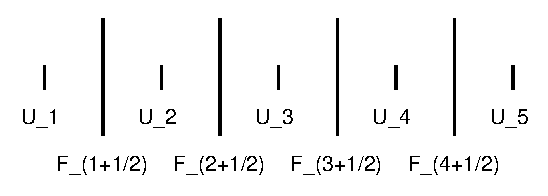
\includegraphics[scale=0.7]{raumaufteilung}
\end{center}
Der 2. Termin (bezeichnet mit $F^v$) entspricht einem künstlichen
Viskositätsterm, der zur Stabilisierung hinzugefügt wurde . Mit
\[
F^v_i = \frac{1}{2 \Delta t}\left(U_i^n - U_{i+1}^n
\right)
\]
folgt für den Beitrag in Gleichung \ref{eq:update_LF}
\[
F^v_{i-1} - F^v_i = \frac{1}{2 \Delta t}\left( U_{i-1} - 2\cdot
U_{i} + U_{i+1} \right) \rightarrow \frac{1}{2}\frac{\Delta
    x^2}{\Delta t} \frac{\partial^2 U}{\partial x^2}
\]
mit
\[
\frac{\partial^2 U}{\partial x^2} = \frac{U_{i+1} - 2\cdot U_{i} +
  U_{i+1} }{\Delta x^2}
\]
Dieser Term verschwindet für kleine Abstände im Raum, da er
proportional zu $\Delta x^2$ ist.

Eine andere und wahrscheinlich einfachere Herleitung ergibt sich durch
die Überlegung, nur mit Mittelwerten über benachbarte Punkte zu
arbeiten. Setzt man in die Gleichung \ref{eq:update_LF} den LF-Fluss
aus Gleichung \ref{eq:fluss_LF} ein, folgt
\begin{eqnarray}
U_i^{n+1} &=& U_i^n + \frac{\Delta t}{\Delta x}\left(
\frac{1}{2}\left(F_{i-1}^n+F_{i}^n \right) + \frac{\Delta x}{2
  \Delta t}\left(U_{i-1}^n - U_{i}^n \right)
-
\frac{1}{2}\left(F_i^n+F_{i+1}^n \right) + \frac{\Delta x}{2
  \Delta t}\left(U_i^n - U_{i+1}^n \right)
\right) \nonumber\\
&=&
U_i^n + \frac{\Delta t}{2\Delta x}
\left(F_{i-1}^n -F_{i+1}^n \right) +
\frac{1}{2} \left(U_{i-1}^n -  2 U_{i}^n + U_{i+1}^n\right) \nonumber\\
&=& \frac{1}{2} \left(U_{i-1}^n + U_{i+1}^n\right)\frac{\Delta t}{2\Delta x}
\left(F_{i-1}^n -F_{i+1}^n \right)
\end{eqnarray}
Das kann so interpretiert werden: Im Raum wird ein zentraler
Differenzenquotient verwendet
\[
\partial_x F_i \rightarrow \frac{F_{i+1} - F_{i-1}}{2\Delta x}
\]
und in der Zeit nicht der ursprüngliche Wert $U_i^n$, sondern der Mittelwert der beiden benachbarten Werte.


Es wurde gezeigt, dass diese Methode stabil ist für eine
CFL-Zahl von $c = 0.9$, siehe Gleichung \ref{eq:cfl}, also  
\[
\Delta t = \frac{\Delta x}{\lambda_{max}} \cdot 0.9
\]

\subsubsection{FORCE Methode}

Im Prinzip kann jeder Form von diskretisiertem Fluss
$\tilde{F}$ verwendet werden, solange für kleine Abstände sich eine
Näherung für die Raumableitung ergibt, also
\[
\lim_{\Delta x \rightarrow 0} \frac{\tilde{F}_{i+1/2}^{n} -
    \tilde{F}_{i-1/2}^{n}} {\Delta x} = \partial_x F(U(x_i,t_n))
\]
Bei der FORCE-Methode wird neben dem Lax-Friedrichs Fluss der
Richtmyer Fluss genommen und ein Mittelwert dieser beiden gemildert. 
Berechne zuerst den einen modifizierten Mittelwert der Variablen
\begin{equation}
U^{RI}_{i+1/2} = \frac{1}{2}\left[U_i^u + U_{i+1}^n\right] + \frac{\Delta t}{2
  \Delta x}\left(F_{i}^n - F_{i+1}^n \right) \label{eq:fluss_RI}
\end{equation}
Das entspricht Gleichung \ref{eq:fluss_LF} des Lax-Friedrichs
Flusses, wobei die Rollen der Variablen und des Flusses vertauscht
sind.  Mit diesen neuen Variablenwerten wird ein Fluss
$F^{RI}_{i+1/2}$ an den Flächen bzw. Mittelpunkten zwischen den
Punkten der Variablen berechnet
\begin{equation}
F^{RI}_{i+1/2} = F(U^{RI}_{i+1/2}) .
\end{equation}
und der Mittelwert zwischen den beiden Flüssen
\begin{equation}
F^{FORCE}_{i+1/2} = \frac{1}{2}\left[ F^{LF}_{i+1/2} +  F^{RI}_{i+1/2} \right]
\end{equation}
wird zum update analog zu Gleichung \ref{eq:update_LF}
\begin{equation}
U_i^{n+1} = U_i^n + \frac{\Delta t}{\Delta x}\left(F^{FORCE}_{i+1/2} -
F^{FORCE}_{i-1/2}\right)
\end{equation}
verwendet.



\subsubsection{Gudanov Methode (NICHT FERTIG!)}

Die sogenannte {\it finite volume Godunov-centered methods} sind genau
die oben vorgestellten Methoden {\it upwind schemes}, die er 1959
entwickelt hat. Sie arbeiten mit der Standardform für ein update
\begin{equation}
U_i^{n+1} = U_i^n + \frac{\Delta t}{\Delta x}\left(F^{Gu}_{i+1/2} -
F^{Gu}_{i-1/2}\right),
\end{equation}
jedoch wird jetzt in den Fluss eine lokale Lösung des Riemanproblems
der Variablen $U$ verwendet.
\[
F^{Gu}_{i+1/2} = F (U_{RP}(0,U_i,u_{i+1})
\]
Ist $w=w(x/t;u_l,u_r)$ eine approximative Lösung des Riemanproblems,
so lässt sich damit der Fluss berechnen. Genaueres kommt später mal,
denn {\bf das Berechnungsschema ist mir noch unklar!}. Prinzip:
\begin{itemize}
\item Beginne mit den initialen Werten
\begin{equation}
U(x,t^n) = \left\{ 
\begin{array}{ll}
U_L & x < x_{i+1/2}\\
U_R & x > x_{i+1/2}\\
\end{array}
\right.
\end{equation}
\end{itemize}
Warum $t^n$ ist unklar.

Weiterhin fehlt auch noch das SLIC-Schema (Slope Limiter Centred).
